% -*- mode: latex; mode: flyspell; ispell-local-dictionary: "en_US"; coding: utf-8; fill-column: 80 -*-

\documentclass[landscape]{article}

\usepackage[utf8]{inputenc}
\usepackage[english]{babel}

\usepackage{amsmath,amsfonts,amssymb}
\usepackage{fullpage}
\usepackage{verbatim}

\usepackage[margin=10mm, top=5mm, bottom=5mm]{geometry}

\usepackage{tikz,pgfplots}

\pgfplotsset{
  width=240mm,height=180mm,
  major grid style={thin,dotted,color=black!50},
  minor grid style={thin,dotted,color=black!50},
  grid,
  every axis/.append style={
    line width=0.5pt,
    tick style={
      line cap=round,
      thin,
      major tick length=4pt,
      minor tick length=2pt,
    },
  },
  legend cell align=left,
  legend pos=north west,
  compat=1.9
}

%%%%%%%%%%%%%%%%%%%%%%%%%%%%%%%%%%%%%%%%%%%%%%%%%%%%%%%%%%%%%%%%%%%%%%%%%%%%%%%%

\begin{document}

% IMPORT-DATA data jobs/job*

\begin{center}

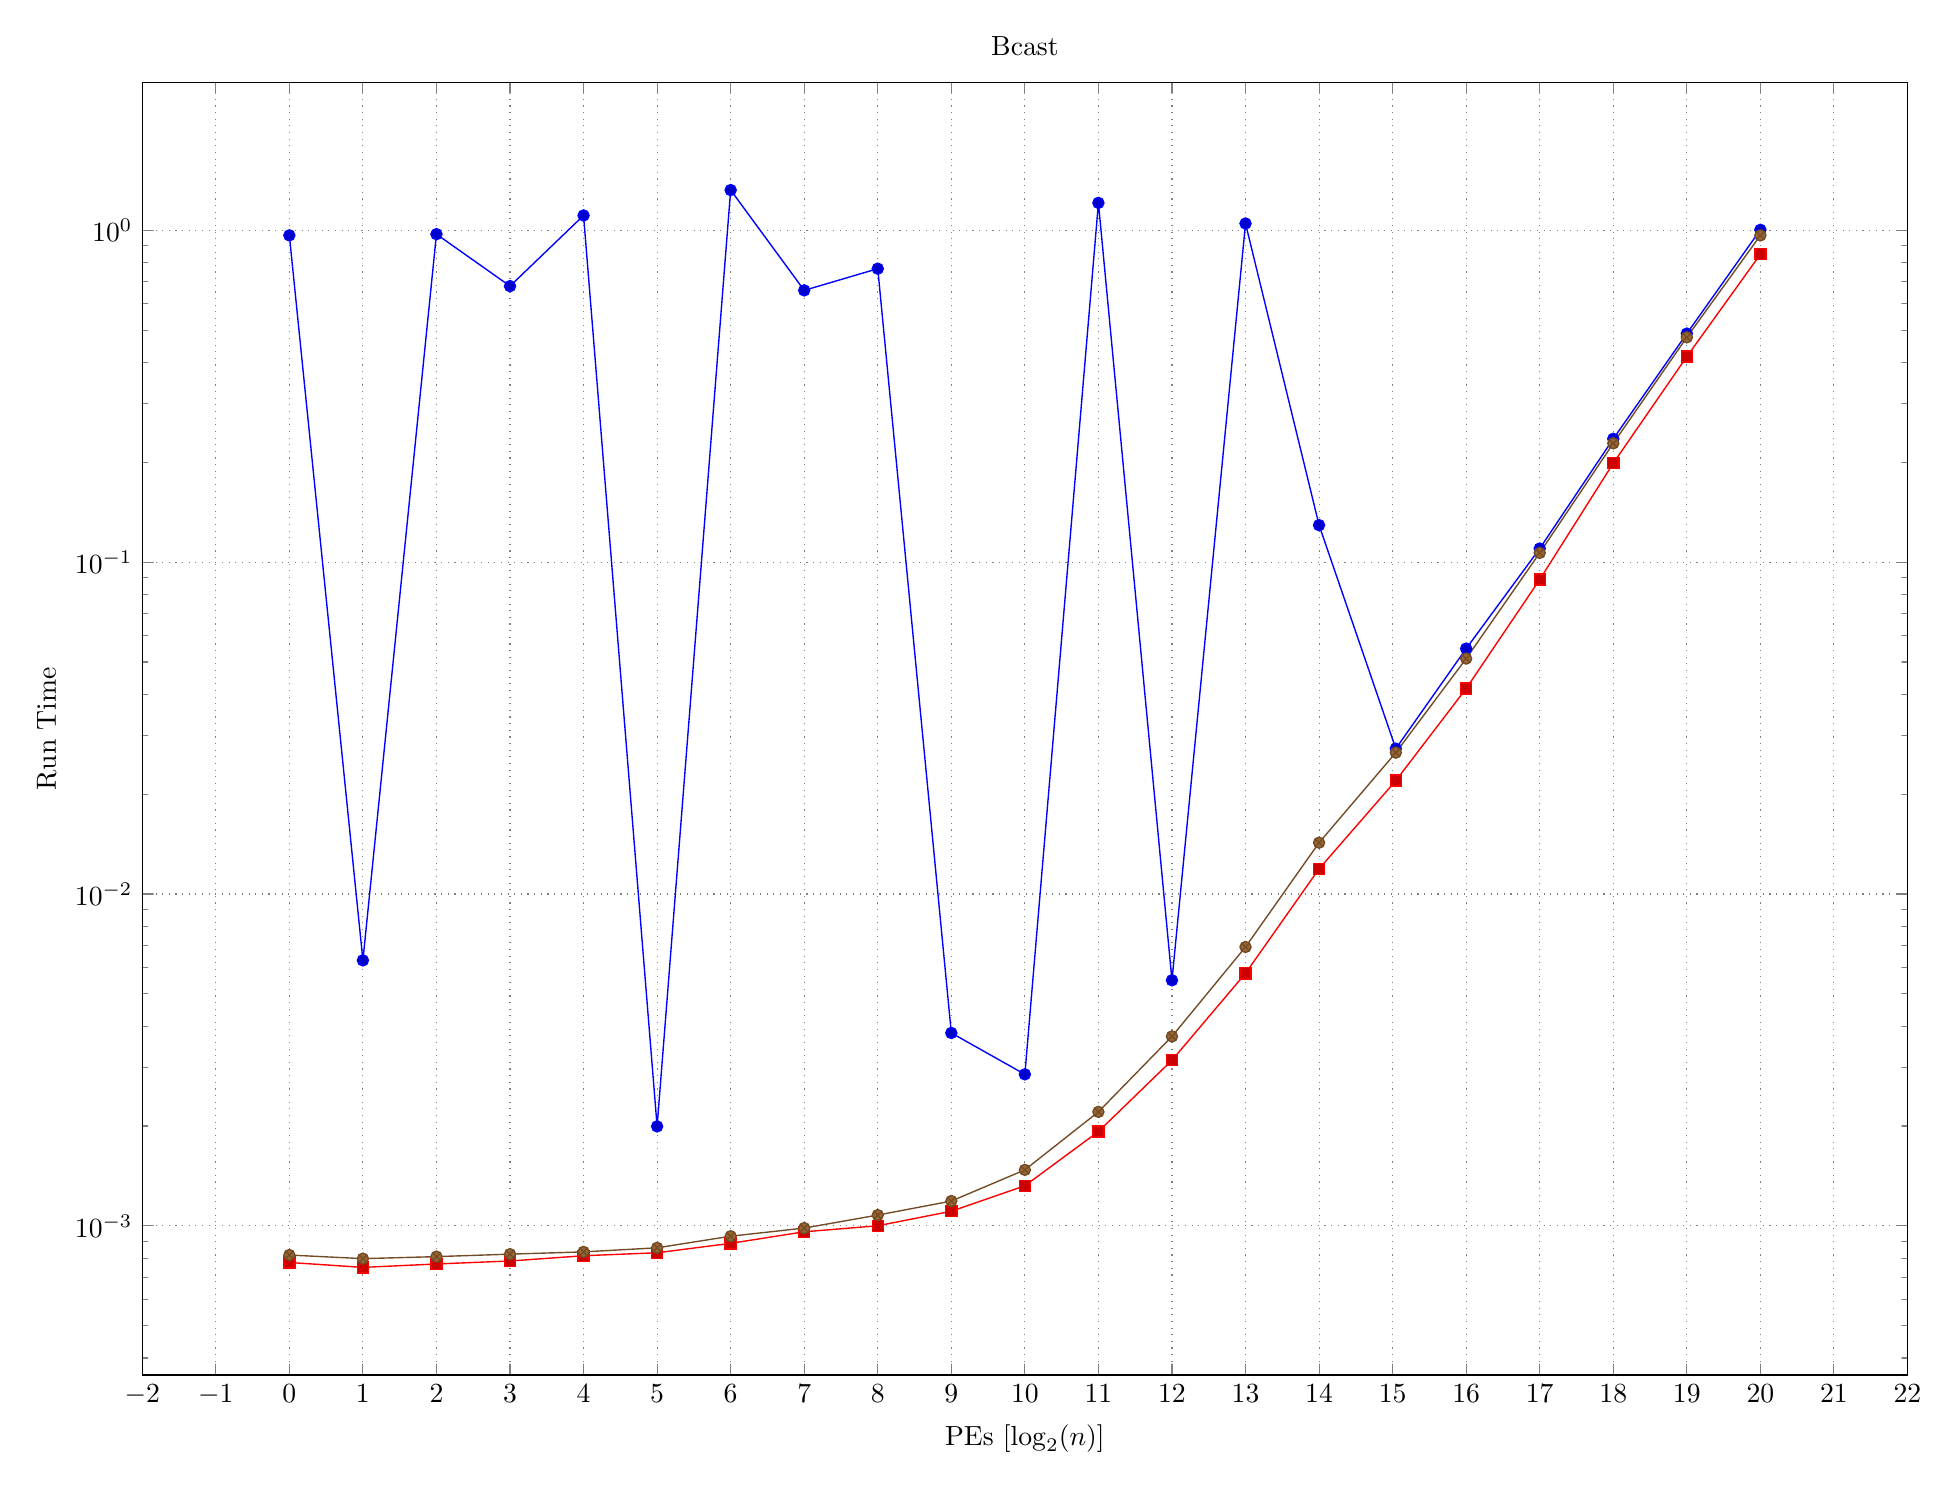
\begin{tikzpicture}
  \begin{axis}[
    title={Bcast},
    ymode=log,
    xlabel={PEs [$\log_2(n)$]},
    ylabel={Run Time},
    ]
    %% PLOT SELECT LOG(2,"n-p") AS x, MAX("wall-time") as y
    %% from data
    %% WHERE algo = 'LightSplitParQsortDistTwoDistSorterMechanism<LightSplitBinTreeKMedianSelect,KNeighborhoodPivotSelectorMechanism>' AND iteration > 0 and p=8192
    %% GROUP BY x  ORDER BY x
    \addplot coordinates { (0,0.964867) (1,0.006311) (2,0.972781) (3,0.678435) (4,1.10757) (5,0.001995) (6,1.320972) (7,0.658732) (8,0.765745) (9,0.003814) (10,0.002862) (11,1.208286) (12,0.005496) (13,1.047443) (14,0.129211) (15.0434,0.027413) (16,0.054869) (17,0.109851) (18,0.235167) (19,0.48805) (20,1.002656) };
    
    %% PLOT SELECT LOG(2,"n-p") AS x, MIN("wall-time") as y
    %% from data
    %% WHERE algo = 'LightSplitParQsortDistTwoDistSorterMechanism<LightSplitBinTreeKMedianSelect,KNeighborhoodPivotSelectorMechanism>' AND iteration > 0 and p=8192
    %% GROUP BY x  ORDER BY x
    \addplot coordinates { (0,0.000776) (1,0.00075) (2,0.000768) (3,0.000784) (4,0.000813) (5,0.00083) (6,0.000886) (7,0.00096) (8,0.001001) (9,0.001107) (10,0.001321) (11,0.001925) (12,0.003156) (13,0.005769) (14,0.011908) (15.0434,0.021959) (16,0.041603) (17,0.088596) (18,0.198655) (19,0.415981) (20,0.846214) };
    
    %% PLOT SELECT LOG(2,"n-p") AS x, MEDIAN("wall-time") as y
    %% from data
    %% WHERE algo = 'LightSplitParQsortDistTwoDistSorterMechanism<LightSplitBinTreeKMedianSelect,KNeighborhoodPivotSelectorMechanism>' AND iteration > 0 and p=8192
    %% GROUP BY x  ORDER BY x
    \addplot coordinates { (0,0.000817) (1,0.000797) (2,0.000808) (3,0.000822) (4,0.000835) (5,0.000859) (6,0.000931) (7,0.000985) (8,0.001078) (9,0.001188) (10,0.001475) (11,0.002206) (12,0.003723) (13,0.006925) (14,0.014276) (15.0434,0.0266645) (16,0.0512005) (17,0.106592) (18,0.227972) (19,0.475533) (20,0.964438) };
  \end{axis}
\end{tikzpicture}

\end{center}

\begin{center}

\begin{tikzpicture}
  \begin{axis}[
    title={Bcast},
    ymode=log,
    xlabel={PEs [$\log_2(n)$]},
    ylabel={Run Time},
    ]
    %% PLOT SELECT LOG(2,"n-p") AS x, MAX("wall-time") as y
    %% from data
    %% WHERE algo = 'LightSplitParQsortDistTwoDistSorterMechanism<LightSplitBinTreeKMedianSelect,KNeighborhoodPivotSelectorMechanism>' AND iteration > 0 and generator='UniformGeneratorMechanism' and p=8192
    %% GROUP BY x  ORDER BY x
    \addplot coordinates { (0,0.964867) (1,0.000937) (2,0.000932) (3,0.000949) (4,0.000986) (5,0.000904) (6,1.086854) (7,0.001048) (8,0.765745) (9,0.001302) (10,0.001515) (11,0.002335) (12,0.004506) (13,0.007638) (14,0.014981) (15.0434,0.027283) (16,0.05157) (17,0.108003) (18,0.235167) (19,0.481697) (20,0.986355) };
    
    %% PLOT SELECT LOG(2,"n-p") AS x, MIN("wall-time") as y
    %% from data
    %% WHERE algo = 'LightSplitParQsortDistTwoDistSorterMechanism<LightSplitBinTreeKMedianSelect,KNeighborhoodPivotSelectorMechanism>' AND iteration > 0 and generator='UniformGeneratorMechanism' and p=8192
    %% GROUP BY x  ORDER BY x
    \addplot coordinates { (0,0.000812) (1,0.000772) (2,0.000782) (3,0.000792) (4,0.00082) (5,0.000839) (6,0.000901) (7,0.000968) (8,0.001077) (9,0.001186) (10,0.001473) (11,0.002216) (12,0.003709) (13,0.006947) (14,0.014115) (15.0434,0.026669) (16,0.051085) (17,0.107188) (18,0.228054) (19,0.47522) (20,0.963587) };
    
    %% PLOT SELECT LOG(2,"n-p") AS x, MEDIAN("wall-time") as y
    %% from data
    %% WHERE algo = 'LightSplitParQsortDistTwoDistSorterMechanism<LightSplitBinTreeKMedianSelect,KNeighborhoodPivotSelectorMechanism>' AND iteration > 0 and generator='UniformGeneratorMechanism' and p=8192
    %% GROUP BY x  ORDER BY x
    \addplot coordinates { (0,0.000824) (1,0.000785) (2,0.000833) (3,0.000821) (4,0.000832) (5,0.000857) (6,0.000965) (7,0.000998) (8,0.001095) (9,0.00122) (10,0.001491) (11,0.002227) (12,0.003785) (13,0.006989) (14,0.014496) (15.0434,0.02685) (16,0.051283) (17,0.107289) (18,0.229763) (19,0.475768) (20,0.970193) };
  \end{axis}
\end{tikzpicture}

\end{center}

\begin{center}

\begin{tikzpicture}
  \begin{axis}[
    title={Bcast},
    ymode=log,
    xlabel={PEs [$\log_2(n)$]},
    ylabel={Run Time},
    ]
    %% PLOT SELECT LOG(2,"n-p") AS x, MAX("wall-time") as y
    %% from data
    %% WHERE algo = 'LightSplitParQsortDistTwoDistSorterMechanism<LightSplitBinTreeKMedianSelect,KNeighborhoodPivotSelectorMechanism>' AND iteration > 0 and generator='SplitCGGroupGeneratorMechanism' and p=8192
    %% GROUP BY x  ORDER BY x
    \addplot coordinates { (0,0.000837) (1,0.000893) (2,0.000844) (3,0.678435) (4,0.000952) (5,0.000859) (6,0.000993) (7,0.001108) (8,0.001108) (9,0.003814) (10,0.00157) (11,0.002432) (12,0.003784) (13,0.007002) (14,0.129211) (15.0434,0.027309) (16,0.052493) (17,0.109341) (18,0.229877) (19,0.478968) (20,0.980961) };
    
    %% PLOT SELECT LOG(2,"n-p") AS x, MIN("wall-time") as y
    %% from data
    %% WHERE algo = 'LightSplitParQsortDistTwoDistSorterMechanism<LightSplitBinTreeKMedianSelect,KNeighborhoodPivotSelectorMechanism>' AND iteration > 0 and generator='SplitCGGroupGeneratorMechanism' and p=8192
    %% GROUP BY x  ORDER BY x
    \addplot coordinates { (0,0.000781) (1,0.000762) (2,0.000785) (3,0.000786) (4,0.000824) (5,0.000842) (6,0.000913) (7,0.000967) (8,0.001031) (9,0.001178) (10,0.001471) (11,0.002207) (12,0.003704) (13,0.006918) (14,0.01415) (15.0434,0.02652) (16,0.050765) (17,0.106223) (18,0.227685) (19,0.475985) (20,0.964113) };
    
    %% PLOT SELECT LOG(2,"n-p") AS x, MEDIAN("wall-time") as y
    %% from data
    %% WHERE algo = 'LightSplitParQsortDistTwoDistSorterMechanism<LightSplitBinTreeKMedianSelect,KNeighborhoodPivotSelectorMechanism>' AND iteration > 0 and generator='SplitCGGroupGeneratorMechanism' and p=8192
    %% GROUP BY x  ORDER BY x
    \addplot coordinates { (0,0.000805) (1,0.000783) (2,0.000792) (3,0.000841) (4,0.000843) (5,0.000852) (6,0.000936) (7,0.000996) (8,0.001088) (9,0.001189) (10,0.00149) (11,0.002225) (12,0.003731) (13,0.006951) (14,0.014312) (15.0434,0.026877) (16,0.05108) (17,0.107129) (18,0.228748) (19,0.477252) (20,0.971122) };
  \end{axis}
\end{tikzpicture}

\end{center}

\newpage

\begin{center}

\begin{tikzpicture}
  \begin{axis}[
    title={Bcast},
    ymode=log,
    xlabel={PEs [$\log_2(n)$]},
    ylabel={Run Time},
    ]
    %% PLOT SELECT LOG(2,"n-p") AS x, MAX("wall-time") as y
    %% from data
    %% WHERE algo = 'SchizoQSDistTwoDistSorterMechanism' AND iteration > 0 and p=8192
    %% GROUP BY x  ORDER BY x
    \addplot coordinates { (0,0.548069) (1,0.701302) (2,0.227613) (3,0.549603) (4,0.235867) (5,0.768698) (6,0.763076) (7,0.836535) (8,0.845712) (9,0.837171) (10,0.854202) (11,0.930969) (12,0.891952) (13,0.996483) (14,1.085228) (15.0434,1.477245) (16,0.950759) (17,1.095203) (18,0.294728) (19,0.539032) (20,1.07053) };
    
    %% PLOT SELECT LOG(2,"n-p") AS x, MIN("wall-time") as y
    %% from data
    %% WHERE algo = 'SchizoQSDistTwoDistSorterMechanism' AND iteration > 0 and p=8192
    %% GROUP BY x  ORDER BY x
    \addplot coordinates { (0,0.002483) (1,0.002364) (2,0.002428) (3,0.002402) (4,0.002463) (5,0.002402) (6,0.002431) (7,0.00242) (8,0.002469) (9,0.002472) (10,0.00246) (11,0.002557) (12,0.002699) (13,0.003161) (14,0.003812) (15.0434,0.005242) (16,0.008119) (17,0.015862) (18,0.047936) (19,0.107052) (20,0.225685) };
    
    %% PLOT SELECT LOG(2,"n-p") AS x, MEDIAN("wall-time") as y
    %% from data
    %% WHERE algo = 'SchizoQSDistTwoDistSorterMechanism' AND iteration > 0 and p=8192
    %% GROUP BY x  ORDER BY x
    \addplot coordinates { (0,0.002801) (1,0.002825) (2,0.002886) (3,0.002964) (4,0.002968) (5,0.003068) (6,0.003098) (7,0.003137) (8,0.003214) (9,0.00343) (10,0.003531) (11,0.00442) (12,0.005753) (13,0.009848) (14,0.069602) (15.0434,0.113627) (16,0.120181) (17,0.136768) (18,0.220649) (19,0.447174) (20,0.88725) };
  \end{axis}
\end{tikzpicture}

\end{center}

\newpage

\begin{center}

\begin{tikzpicture}
  \begin{axis}[
    title={Bcast},
    ymode=log,
    xlabel={PEs [$\log_2(n)$]},
    ylabel={Run Time},
    ]
    %% PLOT SELECT LOG(2,"n-p") AS x, MAX("wall-time") as y
    %% from data
    %% WHERE algo = 'SchizoQSDistTwoDistSorterMechanism' AND iteration > 0 and generator='UniformGeneratorMechanism' and p=8192
    %% GROUP BY x  ORDER BY x
    \addplot coordinates { (0,0.004062) (1,0.015282) (2,0.003729) (3,0.004329) (4,0.004346) (5,0.004461) (6,0.00334) (7,0.003473) (8,0.030484) (9,0.003992) (10,0.006451) (11,0.004873) (12,0.006418) (13,0.013088) (14,0.444136) (15.0434,0.162205) (16,0.216048) (17,0.209415) (18,0.269901) (19,0.500637) (20,0.998021) };
    
    %% PLOT SELECT LOG(2,"n-p") AS x, MIN("wall-time") as y
    %% from data
    %% WHERE algo = 'SchizoQSDistTwoDistSorterMechanism' AND iteration > 0 and generator='UniformGeneratorMechanism' and p=8192
    %% GROUP BY x  ORDER BY x
    \addplot coordinates { (0,0.002715) (1,0.002772) (2,0.002882) (3,0.003067) (4,0.003034) (5,0.003125) (6,0.003086) (7,0.003133) (8,0.003204) (9,0.003277) (10,0.00363) (11,0.004414) (12,0.006026) (13,0.00995) (14,0.069435) (15.0434,0.084618) (16,0.138913) (17,0.13587) (18,0.242087) (19,0.48469) (20,0.950161) };
    
    %% PLOT SELECT LOG(2,"n-p") AS x, MEDIAN("wall-time") as y
    %% from data
    %% WHERE algo = 'SchizoQSDistTwoDistSorterMechanism' AND iteration > 0 and generator='UniformGeneratorMechanism' and p=8192
    %% GROUP BY x  ORDER BY x
    \addplot coordinates { (0,0.002812) (1,0.002985) (2,0.003037) (3,0.00314) (4,0.003168) (5,0.003347) (6,0.003207) (7,0.003297) (8,0.003256) (9,0.003458) (10,0.003857) (11,0.004473) (12,0.006126) (13,0.010111) (14,0.080255) (15.0434,0.135301) (16,0.161376) (17,0.192584) (18,0.264925) (19,0.491658) (20,0.974875) };
  \end{axis}
\end{tikzpicture}

\end{center}

\newpage

\begin{center}

\begin{tikzpicture}
  \begin{axis}[
    title={Bcast},
    ymode=log,
    xlabel={PEs [$\log_2(n)$]},
    ylabel={Run Time},
    ]
    %% PLOT SELECT LOG(2,"n-p") AS x, MAX("wall-time") as y
    %% from data
    %% WHERE algo = 'SchizoQSDistTwoDistSorterMechanism' AND iteration > 0 and generator='SplitCGGroupGeneratorMechanism' and p=8192
    %% GROUP BY x  ORDER BY x
    \addplot coordinates { (0,0.003415) (1,0.002908) (2,0.002763) (3,0.00331) (4,0.00282) (5,0.002672) (6,0.002602) (7,0.003198) (8,0.00322) (9,0.003668) (10,0.003503) (11,0.006406) (12,0.005276) (13,0.008694) (14,0.064174) (15.0434,0.087883) (16,0.068667) (17,0.093787) (18,0.17225) (19,0.348314) (20,0.713596) };
    
    %% PLOT SELECT LOG(2,"n-p") AS x, MIN("wall-time") as y
    %% from data
    %% WHERE algo = 'SchizoQSDistTwoDistSorterMechanism' AND iteration > 0 and generator='SplitCGGroupGeneratorMechanism' and p=8192
    %% GROUP BY x  ORDER BY x
    \addplot coordinates { (0,0.002529) (1,0.002467) (2,0.002441) (3,0.002402) (4,0.002473) (5,0.002443) (6,0.002461) (7,0.003018) (8,0.002999) (9,0.003061) (10,0.003298) (11,0.003863) (12,0.005194) (13,0.00816) (14,0.027681) (15.0434,0.052802) (16,0.054169) (17,0.081396) (18,0.166983) (19,0.337701) (20,0.698786) };
    
    %% PLOT SELECT LOG(2,"n-p") AS x, MEDIAN("wall-time") as y
    %% from data
    %% WHERE algo = 'SchizoQSDistTwoDistSorterMechanism' AND iteration > 0 and generator='SplitCGGroupGeneratorMechanism' and p=8192
    %% GROUP BY x  ORDER BY x
    \addplot coordinates { (0,0.002605) (1,0.002531) (2,0.002522) (3,0.002514) (4,0.002535) (5,0.002513) (6,0.002545) (7,0.003105) (8,0.003187) (9,0.003207) (10,0.003399) (11,0.004015) (12,0.005235) (13,0.008252) (14,0.043537) (15.0434,0.056527) (16,0.06254) (17,0.089267) (18,0.169318) (19,0.342274) (20,0.709805) };
  \end{axis}
\end{tikzpicture}

\end{center}

\newpage

\begin{center}

\begin{tikzpicture}
  \begin{axis}[
    title={Bcast},
    ymode=log,
    xlabel={PEs [$\log_2(n)$]},
    ylabel={Run Time},
    ]
    %% PLOT SELECT LOG(2,"n-p") AS x, MAX("wall-time") as y
    %% from data
    %% WHERE algo = 'SchizoQSDistTwoDistSorterMechanism' AND iteration > 0 and generator='UniformGeneratorMechanism' and p=16384
    %% GROUP BY x  ORDER BY x
    \addplot coordinates { (0,0.003606) (1,0.003711) (2,0.004575) (3,1.863242) (4,0.003981) (5,0.004379) (6,0.004333) (7,0.004344) (8,0.004972) (9,0.004564) (10,0.004745) (11,0.00584) (12,0.00789) (13,0.013094) (14,0.090917) (15.0434,1.122408) (16,0.228752) (17,0.26604) (18,0.369603) (19,0.648638) (20,1.271673) };
    
    %% PLOT SELECT LOG(2,"n-p") AS x, MIN("wall-time") as y
    %% from data
    %% WHERE algo = 'SchizoQSDistTwoDistSorterMechanism' AND iteration > 0 and generator='UniformGeneratorMechanism' and p=16384
    %% GROUP BY x  ORDER BY x
    \addplot coordinates { (0,0.00324) (1,0.003521) (2,0.003773) (3,0.004135) (4,0.003795) (5,0.003878) (6,0.003947) (7,0.003914) (8,0.00408) (9,0.004165) (10,0.004506) (11,0.005558) (12,0.007805) (13,0.012286) (14,0.085145) (15.0434,0.168756) (16,0.153888) (17,0.226157) (18,0.351041) (19,0.620042) (20,1.237128) };
    
    %% PLOT SELECT LOG(2,"n-p") AS x, MEDIAN("wall-time") as y
    %% from data
    %% WHERE algo = 'SchizoQSDistTwoDistSorterMechanism' AND iteration > 0 and generator='UniformGeneratorMechanism' and p=16384
    %% GROUP BY x  ORDER BY x
    \addplot coordinates { (0,0.003398) (1,0.003671) (2,0.00384) (3,0.004275) (4,0.003881) (5,0.003887) (6,0.003966) (7,0.003996) (8,0.004457) (9,0.004329) (10,0.004541) (11,0.005575) (12,0.007839) (13,0.012767) (14,0.086386) (15.0434,0.652325) (16,0.22183) (17,0.241781) (18,0.358315) (19,0.641258) (20,1.260968) };
  \end{axis}
\end{tikzpicture}

\end{center}

\end{document}

%%%%%%%%%%%%%%%%%%%%%%%%%%%%%%%%%%%%%%%%%%%%%%%%%%%%%%%%%%%%%%%%%%%%%%%%%%%%%%%%
